\documentclass[aspectratio=169,11pt]{beamer}
\usetheme{Madrid}
\usecolortheme{default}
\usepackage{graphicx}
\usepackage{booktabs}
\usepackage{hyperref}
\usepackage{tikz}
\usepackage{colortbl}
\usetikzlibrary{arrows.meta,positioning,shapes.geometric}

\definecolor{darkblue}{RGB}{0,51,102}
\definecolor{lightblue}{RGB}{51,122,183}
\definecolor{accentgreen}{RGB}{40,167,69}
\definecolor{accentred}{RGB}{200,50,50}
\setbeamercolor{structure}{fg=darkblue}
\setbeamercolor{title}{fg=white,bg=darkblue}
\setbeamercolor{frametitle}{fg=white,bg=darkblue}
\setbeamercolor{block title}{fg=white,bg=lightblue}

\setbeamertemplate{navigation symbols}{}
\setbeamertemplate{footline}{
  \leavevmode\hbox{%
    \begin{beamercolorbox}[wd=.333\paperwidth,ht=2.5ex,dp=1ex,center]{author in head/foot}%
      \usebeamerfont{author in head/foot}\insertshortauthor
    \end{beamercolorbox}%
    \begin{beamercolorbox}[wd=.334\paperwidth,ht=2.5ex,dp=1ex,center]{title in head/foot}%
      \usebeamerfont{title in head/foot}MIE1512 --- Prof.\ Consens
    \end{beamercolorbox}%
    \begin{beamercolorbox}[wd=.333\paperwidth,ht=2.5ex,dp=1ex,right]{date in head/foot}%
      \usebeamerfont{date in head/foot}\insertframenumber{} / \inserttotalframenumber\hspace*{2ex}
    \end{beamercolorbox}}%
}

\title[LLM Judgment vs Human Preference]{Can LLM Judgment Capture Human Preference?}
\subtitle{An Alignment Study Between Automated and Human\\Evaluation of LLM Task Performance}
\author[Yifan Liu]{Yifan Liu \\ {\small Student \#1007341681}}
\institute[UofT]{Department of Mechanical and Industrial Engineering\\University of Toronto}
\date{March 2026}

\begin{document}

% ============================
\begin{frame}
\titlepage
\end{frame}

% ============================
\begin{frame}{Outline}
\tableofcontents
\end{frame}

% ============================
\section{Research Problem}
% ============================

\begin{frame}{The Research Problem}

Evaluating LLMs is expensive. \textbf{Human evaluation} (crowdsourced voting) is the gold standard --- but slow and costly to scale.

\vspace{0.5em}
A popular alternative: use a \textbf{strong LLM as a judge} to evaluate other LLMs automatically.

\vspace{0.8em}
\begin{block}{Research Question}
\textbf{Can an LLM judge reliably capture human preferences when evaluating LLM task performance?}
\end{block}

\vspace{0.5em}
Existing work reports high overall agreement ($r \geq 0.94$) between automated LLM judges and human voters.

\vspace{0.5em}
\textbf{But is this agreement uniform?} Or does the LLM judge agree with humans on some tasks and fail on others?
\end{frame}

% ============================
\begin{frame}{Why This Matters}

\begin{enumerate}
    \item \textbf{Replacing human evaluation}\\
    If LLM judges fail on certain task types, using them as a blanket replacement for human evaluation is unreliable.

    \vspace{0.5em}
    \item \textbf{Model development}\\
    RLHF, DPO, and other alignment methods use automated scores as training signals. If the automated judge disagrees with humans on math or translation, models trained on those signals may be optimized for the wrong objective.

    \vspace{0.5em}
    \item \textbf{Model selection}\\
    Practitioners choose LLMs based on benchmark leaderboards. If the leaderboard is driven by an LLM judge that doesn't match human preferences for their use case, they may pick the wrong model.
\end{enumerate}
\end{frame}

% ============================
\section{Method: LLM-as-Judge}
% ============================

\begin{frame}{LLM-as-Judge: How It Works}

The \textbf{LLM-as-judge} paradigm uses a strong LLM (e.g., GPT-4-turbo) to automatically evaluate outputs from other models, replacing expensive human annotation.

\vspace{0.5em}
\textbf{WildBench} (Lin et al., ICLR 2025 Spotlight) is a leading implementation:

\vspace{0.3em}
\begin{columns}[T]
\begin{column}{0.55\textwidth}
\begin{enumerate}\small
    \item \textbf{Input}: A real-user prompt + model response
    \item \textbf{Checklist generation}: GPT-4-turbo generates a \textbf{task-specific checklist} (e.g., code correctness, efficiency, explanation quality for coding tasks)
    \item \textbf{Pointwise scoring (WB-Score)}: Rate the response 1--10 against the checklist
    \item \textbf{Pairwise scoring (WB-Reward)}: Compare response against 3 reference models with 5 outcome levels, corrected for length bias
\end{enumerate}
\end{column}
\begin{column}{0.42\textwidth}
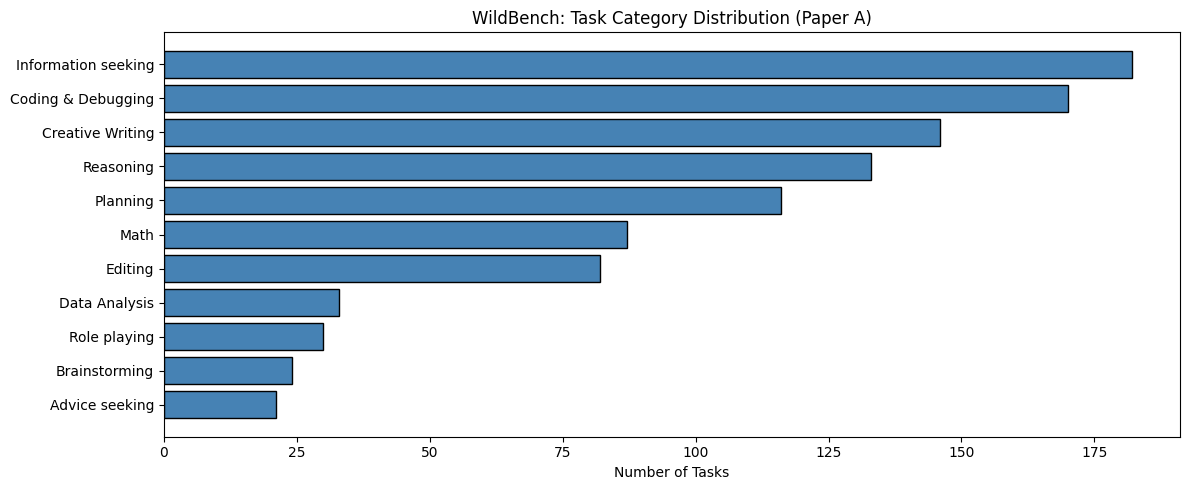
\includegraphics[width=\textwidth]{figures/wb_categories.png}

\vspace{0.2em}
{\scriptsize 1,024 tasks across 12 categories, 60+ models evaluated. Reports $r = 0.98$ with human Elo.}
\end{column}
\end{columns}
\end{frame}

% ============================
\begin{frame}{Task-Specific Checklists: The Key Idea}

What makes WildBench different from naive LLM-as-judge is the \textbf{task-specific checklist}:

\vspace{0.5em}
\begin{columns}[T]
\begin{column}{0.48\textwidth}
\begin{block}{Coding \& Debugging}
\begin{itemize}\small
    \item Does the code compile/run?
    \item Is the logic correct?
    \item Are edge cases handled?
    \item Is the code efficient?
\end{itemize}
\end{block}

\begin{block}{Creative Writing}
\begin{itemize}\small
    \item Is the narrative engaging?
    \item Is the tone appropriate?
    \item Is the language fluent and vivid?
\end{itemize}
\end{block}
\end{column}
\begin{column}{0.48\textwidth}
\begin{block}{Mathematics}
\begin{itemize}\small
    \item Is the final answer correct?
    \item Are intermediate steps valid?
    \item Is the reasoning complete?
\end{itemize}
\end{block}

\begin{block}{Translation}
\begin{itemize}\small
    \item Is the meaning preserved?
    \item Is the grammar correct?
    \item Are cultural nuances handled?
\end{itemize}
\end{block}
\end{column}
\end{columns}

\vspace{0.5em}
This categorization into \textbf{12 task types} is central to our analysis --- we apply it to human preference data to test per-category agreement.
\end{frame}

% ============================
\section{Dataset: Chatbot Arena}
% ============================

\begin{frame}{Chatbot Arena: Human Preference at Scale}

{\small Chiang et al., ICML 2024}

\vspace{0.3em}
The largest open human preference dataset for LLM evaluation:

\vspace{0.3em}
\begin{columns}[T]
\begin{column}{0.55\textwidth}
\begin{itemize}\small
    \item A user submits a prompt and sees responses from \textbf{two anonymous LLMs} side by side
    \item The user votes for the response they prefer
    \item \textbf{57,477 pairwise battles}, 64 models
    \item Full text of prompts and responses available
    \item Supplemented by \textbf{1.7M voting records}
\end{itemize}

\vspace{0.3em}
Rankings computed via \textbf{Bradley-Terry model} $\to$ Elo ratings (same concept as chess). Widely considered the \textbf{gold standard} for alignment evaluation.

\vspace{0.3em}
\textit{This is our ground truth: what do humans actually prefer?}
\end{column}
\begin{column}{0.42\textwidth}
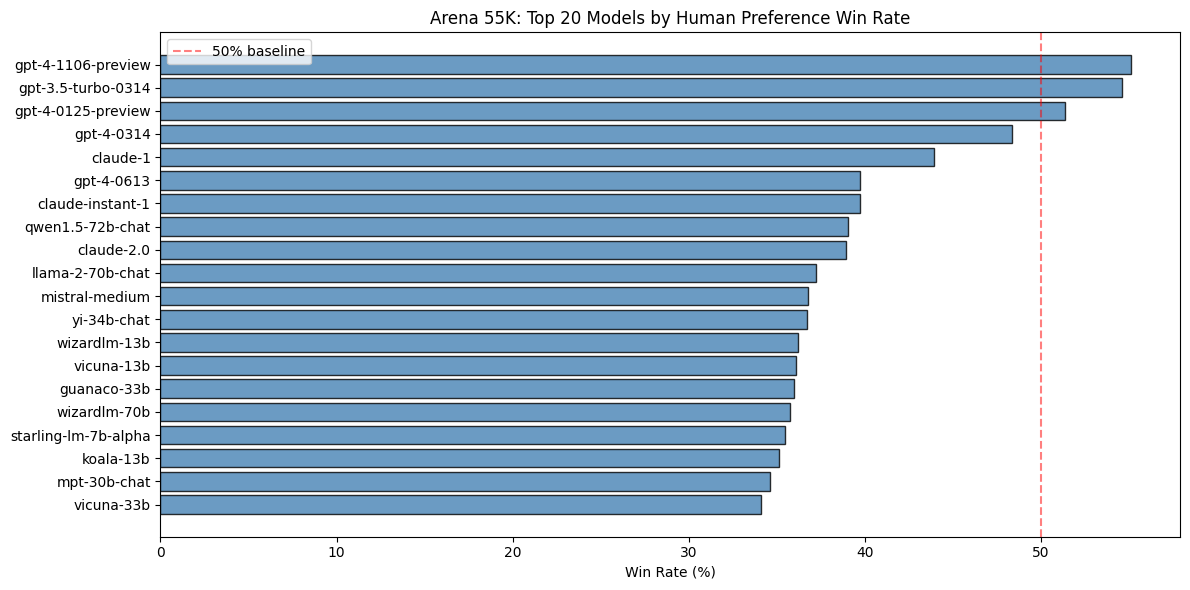
\includegraphics[width=\textwidth]{figures/arena_top20.png}

\vspace{0.2em}
{\scriptsize Top 20 models by Elo (Arena 55K, Bradley-Terry with bootstrap).}
\end{column}
\end{columns}
\end{frame}

% ============================
\begin{frame}{Applying Task Categorization to Arena Data}

Arena provides aggregate Elo rankings but \textbf{no task-category breakdown}. We add one:

\vspace{0.5em}
\begin{center}
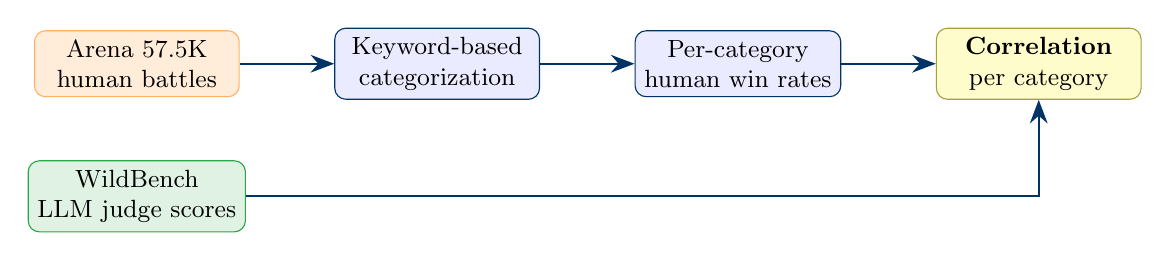
\begin{tikzpicture}[
    node distance=0.6cm and 1.0cm,
    box/.style={rectangle, draw=darkblue, fill=blue!8, rounded corners, minimum width=2.6cm, minimum height=0.8cm, align=center, font=\small},
    arrow/.style={-{Stealth[length=3mm]}, thick, darkblue}
]
    \node[box, fill=orange!15, draw=orange!60] (arena) {Arena 57.5K\\human battles};
    \node[box, right=1.2cm of arena] (classify) {Keyword-based\\categorization};
    \node[box, right=1.2cm of classify] (winrate) {Per-category\\human win rates};
    \node[box, below=0.8cm of arena, fill=accentgreen!15, draw=accentgreen] (wb) {WildBench\\LLM judge scores};
    \node[box, right=1.2cm of winrate, fill=yellow!20, draw=yellow!60!black] (corr) {\textbf{Correlation}\\per category};

    \draw[arrow] (arena) -- (classify);
    \draw[arrow] (classify) -- (winrate);
    \draw[arrow] (winrate) -- (corr);
    \draw[arrow] (wb) -| (corr);
\end{tikzpicture}
\end{center}

\vspace{0.3em}
\begin{itemize}\small
    \item Classify each Arena prompt into WildBench's 12 task types via keyword heuristics (e.g., ``code'', ``debug'', ``Python'' $\to$ Coding \& Debugging)
    \item Compute per-model human win rates within each category
    \item Compare against WildBench's LLM judge scores for \textbf{12 overlapping models}
    \item All processed with PySpark ($\sim$1.8M records). \textbf{No LLM inference} --- all judgments precomputed.
\end{itemize}
\end{frame}

% ============================
\section{Results}
% ============================

\begin{frame}{Result 1: Overall --- the LLM Judge Agrees with Humans}

\begin{columns}[T]
\begin{column}{0.45\textwidth}
{\small Cross-benchmark correlation\\(12 overlapping models):}

\vspace{0.3em}
{\small
\begin{tabular}{@{}lcc@{}}
\toprule
& \textbf{Pearson} & \textbf{Spearman} \\
\midrule
Elo vs WB-Score & \textbf{0.954} & 0.923 \\
Elo vs WB-Reward & \textbf{0.943} & 0.895 \\
\bottomrule
\end{tabular}
}

\vspace{0.5em}
High overall agreement ($p < 10^{-5}$), partly driven by large inter-model gaps --- every benchmark can tell GPT-4 from Llama-2.

\vspace{0.5em}
\textit{This confirms previous findings. But the story changes when we look per category\ldots}
\end{column}

\begin{column}{0.52\textwidth}
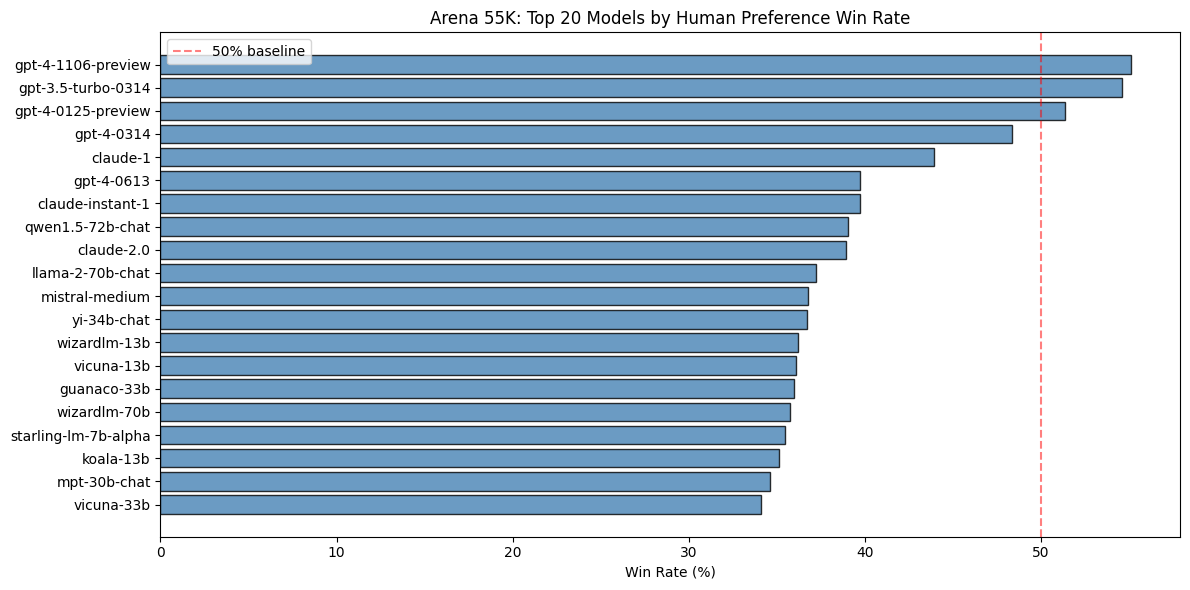
\includegraphics[width=\textwidth]{figures/arena_top20.png}
{\small\centering Top 20 models by human preference\\(Arena 55K, Bradley-Terry Elo)}
\end{column}
\end{columns}
\end{frame}

% ============================
\begin{frame}{Result 2: Per Category --- Agreement Varies Dramatically}

\begin{table}
\centering\small
\begin{tabular}{@{}lccc@{}}
\toprule
\textbf{Task Category} & \textbf{N} & \textbf{Pearson (WB-Score)} & \textbf{Pearson (WB-Reward)} \\
\midrule
\rowcolor{accentgreen!15} Reasoning & 11 & \textbf{0.749} & 0.693 \\
\rowcolor{accentgreen!10} Creative Writing & 11 & 0.713 & 0.649 \\
Coding \& Debugging & 12 & 0.689 & 0.661 \\
Role-Playing & 11 & 0.689 & 0.642 \\
\rowcolor{accentred!10} Information Seeking & 12 & 0.595 & 0.554 \\
Mathematics & 11 & 0.558 & 0.581 \\
\rowcolor{accentred!15} Translation & 5 & \textbf{0.146} & 0.144 \\
\midrule
\textit{Overall} & 12 & \textit{0.954} & \textit{0.943} \\
\bottomrule
\end{tabular}
\end{table}

\vspace{0.3em}
The 0.95 overall correlation \textbf{masks a range from 0.75 to 0.15}. The LLM judge captures human preferences well for reasoning, but \textbf{poorly for translation and mathematics}.
\end{frame}

% ============================
\begin{frame}{Result 3: Human Rankings Shift Across Categories}

\begin{center}
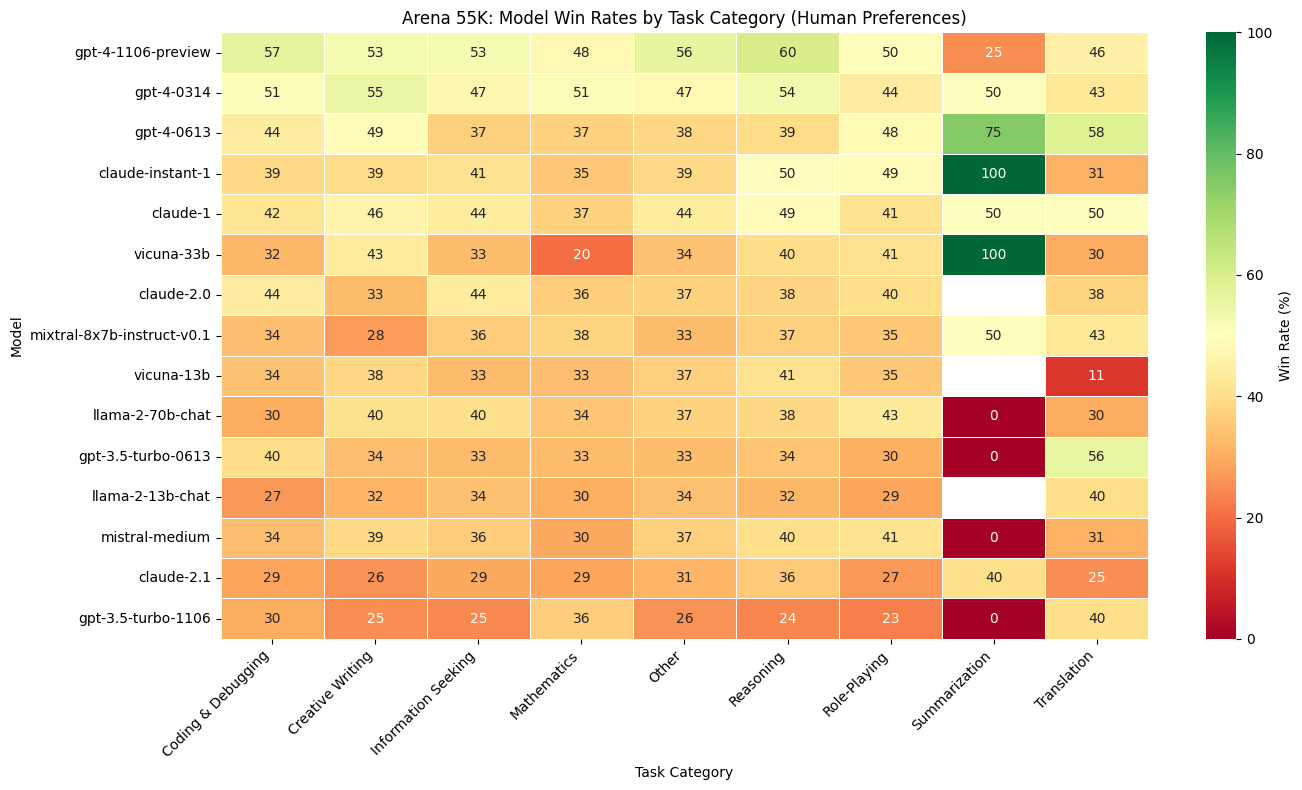
\includegraphics[width=0.78\textwidth]{figures/arena_heatmap.png}
\end{center}
{\small Per-category human preference win rates (Arena 55K, top 15 models). The overall \#1 model (gpt-4-1106-preview) is \textbf{not \#1 in most categories}. Different models lead in different task types.}
\end{frame}

% ============================
\begin{frame}{Result 3 (cont'd): Category-Specific Leaders}

{\small
\begin{tabular}{@{}llr@{}}
\toprule
\textbf{Task Category} & \textbf{Top Model (human votes)} & \textbf{Win Rate} \\
\midrule
Coding \& Debugging & gpt-3.5-turbo-0314 & 61.2\% \\
Creative Writing & gpt-3.5-turbo-0314 & 61.7\% \\
Information Seeking & gpt-3.5-turbo-0314 & 60.0\% \\
Reasoning & \textbf{gpt-4-1106-preview} & 60.2\% \\
Mathematics & gpt-3.5-turbo-0314 & 75.0\% \\
Role-Playing & mpt-30b-chat & 70.0\% \\
Translation & gpt-4-0613 & 58.3\% \\
\bottomrule
\end{tabular}
}

\vspace{0.5em}
\begin{block}{Implication}
A single leaderboard ranking --- whether from an LLM judge or human Elo --- does not tell the full story. The ``best'' model depends on the task. An LLM judge that agrees with humans overall may give \textbf{misleading guidance} for specific use cases.
\end{block}
\end{frame}

% ============================
\section{Summary \& Ongoing Work}
% ============================

\begin{frame}{Summary}

\textbf{Research question}: Can an LLM judge reliably capture human preferences when evaluating LLM task performance?

\vspace{0.5em}
\textbf{Answer}: \textit{It depends on the task.}

\vspace{0.5em}
\begin{enumerate}
    \item \textbf{Overall}: Yes --- LLM judge scores correlate strongly with human Elo ($r = 0.95$).

    \vspace{0.3em}
    \item \textbf{Per category}: Agreement ranges from $r = 0.75$ (reasoning) to $r = 0.15$ (translation). The LLM judge is a reliable proxy for some tasks but not others.

    \vspace{0.3em}
    \item \textbf{Rankings shift}: The best model overall is not the best in most categories. Aggregate scores --- from either LLM judges or human Elo --- hide task-specific strengths and weaknesses.
\end{enumerate}

\vspace{0.5em}
\textbf{Takeaway}: High overall correlation between LLM judges and humans should not be taken as blanket validation. Per-category analysis is necessary.
\end{frame}

% ============================
\begin{frame}{Ongoing Work}

\textbf{Completed}:
\begin{itemize}
    \item[\checkmark] Arena 57.5K: task categorization, per-category human win rates
    \item[\checkmark] Elo ratings via Bradley-Terry model
    \item[\checkmark] Cross-benchmark correlation --- overall and per category (7 categories)
    \item[\checkmark] 7 visualizations: heatmaps, scatter plots, bar charts
\end{itemize}

\vspace{0.5em}
\textbf{In progress}:
\begin{enumerate}
    \item Per-category Elo (fairer than win rate for uneven matchup pools)
    \item 1.7M Arena voting records for more robust Elo estimates
    \item AlpacaEval 2 integration for three-way comparison
    \item Bootstrap confidence intervals for correlation estimates
    \item Improved categorization coverage (currently 40\% of prompts classified)
    \item Full PySpark pipeline at scale
\end{enumerate}
\end{frame}

% ============================
\begin{frame}{}
\vfill
\begin{center}
{\Large\textbf{Thank You}}

\vspace{1em}
{\large Questions?}

\vspace{2em}
{\small
\textbf{References}:\\[0.3em]
Lin et al., ``WildBench: Benchmarking LLMs with Challenging Tasks from Real Users in the Wild,'' ICLR 2025\\[0.2em]
Chiang et al., ``Chatbot Arena: An Open Platform for Evaluating LLMs by Human Preference,'' ICML 2024\\[0.2em]
Dubois et al., ``Length-Controlled AlpacaEval: A Simple Way to Debias Automatic Evaluators,'' COLM 2024
}
\end{center}
\vfill
\end{frame}

\end{document}
